\documentclass{beamer}

\usepackage[utf8]{inputenc}
\usepackage{avant}

\setbeamercovered{transparent}
\setbeamertemplate{navigation symbols}

\setbeamertemplate{footline}{\makebox[0.98\paperwidth][r]{\large \raisebox{1.2ex}{\insertframenumber}}}

\title{DNSKEY Management}

\author{Julien Perrochet \and Tobias Schlatter}
\date{December 12, 2012}
\institute{ITSEC, EPFL, Prof. Janson}

\graphicspath{{../figures/}}

\begin{document}

\begin{frame}
  \titlepage
\end{frame}

\section{Outline}
\begin{frame}
  \frametitle{Outline}

  \begin{block}{Introduction}
  \end{block}

  \begin{block}{Current DNSSEC Deployment}
  \end{block}

  \begin{block}{DNSKEY Management}
  \end{block}

  \begin{block}{Case-Study: Switzerland}
  \end{block}

\end{frame}

\section{Introduction}
\begin{frame}
  \frametitle{DNSSEC Chain of Trust}
  \framesubtitle{How are DNSKEYs verified?}

  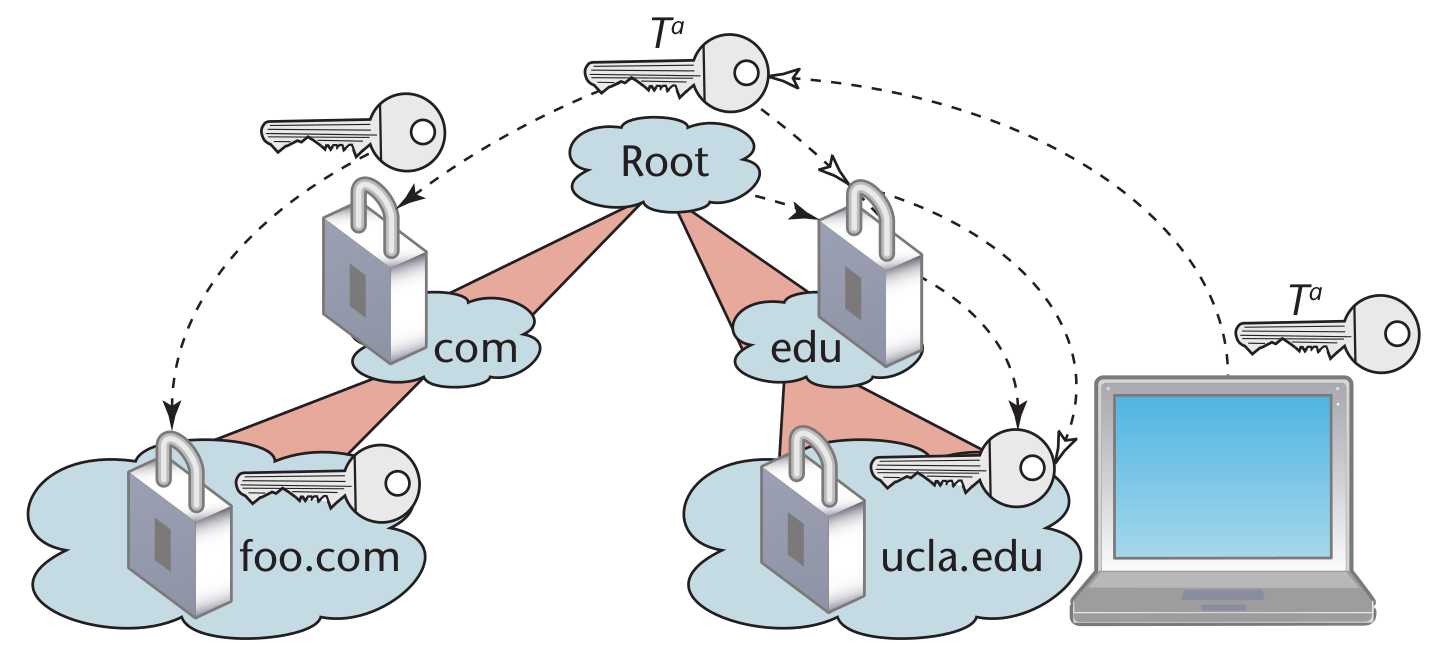
\includegraphics[width=\textwidth]{trust-chain}

\end{frame}



\section{DNSSEC Deployment}

\begin{frame}
  \frametitle{DNSSEC Production Zones}
  \framesubtitle{How many DNSSEC zones are deployed?}
  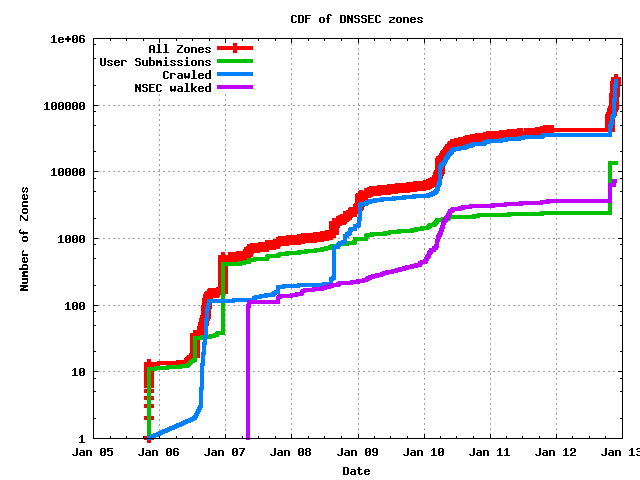
\includegraphics[width=.9\textwidth]{dnssec-growth}
\end{frame}

\begin{frame}
  \frametitle{DNSSEC Certificate Chain}
  \framesubtitle{How many are properly signed?}

  \begin{columns}[c]
    \begin{column}{4.8cm}

      \begin{block}{Root Zone}
        \begin{itemize}
        \item Signed July 15, 2010
        \item $< 50\%$ zones properly chained
        \end{itemize}
      \end{block}
  
      \begin{block}<3->{Trust Anchor Repository}
        \begin{itemize}
        \item Stores trusted keys
        \item Orthogonal to DNSSEC key chain
        \end{itemize}
      \end{block}

    \end{column}

    \begin{column}{6cm}
      \includegraphics<1>  [width=\textwidth]{trust-chain-part}
      \includegraphics<2-3>[width=\textwidth]{trust-chain-no-tar}
      \includegraphics<4>  [width=\textwidth]{trust-chain-tar}
    \end{column}

  \end{columns}

  %% Mention TARs
\end{frame}

\section{Operations}

\begin{frame}
  \frametitle{DNSKEY Operations}
  \framesubtitle{What are the major operations?}

  \begin{columns}[c]
    \begin{column}{4.8cm}
      \begin{block}<1->{Enable DNSSEC}
        \begin{itemize}
        \item Generate key
        \item Parent signs key
        \end{itemize}
      \end{block}

      \begin{block}<4->{Key Rollover}
        \begin{itemize}
        \item Generate new key
        \item Parent signs key
        \item Remove old key
        \end{itemize}
      \end{block}

      \begin{block}<8->{Disable DNSSEC}
        \begin{itemize}
        \item Remove \alert{all} refs to key
        \end{itemize}
      \end{block}

    \end{column}

    \begin{column}{6cm}
      \includegraphics<1>  [width=\textwidth]{trust-chain-ops-1}
      \includegraphics<2>  [width=\textwidth]{trust-chain-ops-2}
      \includegraphics<3,4>[width=\textwidth]{trust-chain-ops-3}
      \includegraphics<5>  [width=\textwidth]{trust-chain-ops-4}
      \includegraphics<6>  [width=\textwidth]{trust-chain-ops-5}
      \includegraphics<7,8>[width=\textwidth]{trust-chain-ops-6}
      \includegraphics<9>  [width=\textwidth]{trust-chain-ops-7}
      \includegraphics<10> [width=\textwidth]{trust-chain-ops-1}
      \includegraphics<11> [width=\textwidth]{trust-chain-tar-no-key}
      \includegraphics<12> [width=\textwidth]{trust-chain-tar-no-deleg}
    \end{column}

  \end{columns}

\end{frame}

\section{Case-Study: CH}

\begin{frame}
  \frametitle{Situation in Switzerland}
  \framesubtitle{
\includegraphics[width=2.6cm]{SWITCH-logo}}

  \begin{block}{Deployment}
    \begin{itemize}
    \item \texttt{ch.} zone securely delegated
    \item Very low penetration (370 / 1.7 mio.)
    \item DNSSEC for free
    \end{itemize}
  \end{block}

  \pause

  \begin{block}{Key Management}
    \begin{itemize}
    \item Enable/Disable keys in web-interface
    \item Partners (Registrars): EPP
    \end{itemize}
  \end{block}
\end{frame}

\section{Conclusion}

\begin{frame}
  \frametitle{Conclusion}
  
  \begin{block}{Comments}
    \begin{itemize}
    \item Most management issues solved
    \item DNSKEY management not relevant enough for course
    \end{itemize}
  \end{block}

  \pause

  \begin{block}{¿Questions?}
  \end{block}
  
\end{frame}

\end{document}

%%% Local Variables: 
%%% mode: latex
%%% TeX-master: t
%%% End: 
